\section{Lab: Networking}

\subsection{实验目的}

本实验将编写一个在xv6操作系统中用于网络接口卡(network interface card, NIC)的设备驱动程序。通过这个实验学习如何初始化并操作一个虚拟的网络设备,以及如何处理网络通信,从而深入理解操作系统中设备驱动程序的工作原理。

本实验将使用一个名为 E1000 的网络设备来处理网络通信。对于 xv6来说,E1000 看起来就像一个连接到真实以太网局域网(LAN)的真实硬件。

\subsection{实验步骤}

在e1000.c文件中完善e1000\_transmit和e1000\_recv函数以实现网卡驱动的功能。

\subsubsection*{e1000\_transmit函数}
e1000\_transmit 函数的作用是将一个数据缓冲区(mbuf)通过 e1000 网卡发送出去。它首先获取一个自旋锁以确保线程安全,然后读取当前的发送描述符索引(TDT)。接着检查对应的发送描述符是否已经被处理,如果未处理则返回错误。否则,将新数据缓冲区的地址和长度写入发送描述符,并设置相关的命令和状态位,通知网卡发送该数据包。最后,更新发送描述符索引(TDT),释放锁并返回成功标志。


\begin{lstlisting}[language=c,title=e1000\_transmit函数的实现]
    int e1000_transmit(struct mbuf *m)
    {
        // 获取e1000锁,确保对发送环形缓冲区的访问是安全的
        acquire(&e1000_lock);

        // 获取当前TDT(发送描述符尾部指针)的值,即网卡硬件当前处理到的发送描述符索引
        uint64 tdt = regs[E1000_TDT];
        // 计算发送环中的当前索引
        uint64 index = tdt % TX_RING_SIZE;
        // 获取当前索引处的发送描述符
        struct tx_desc send_desc = tx_ring[index];

        // 检查发送描述符是否已经被硬件处理(通过判断状态位是否包含DD标志)
        if (!(send_desc.status & E1000_TXD_STAT_DD))
        {
            // 如果发送描述符尚未处理,说明环形缓冲区满,释放锁并返回-1表示失败
            release(&e1000_lock);
            return -1;
        }

        // 如果之前存在缓冲区,则释放它
        if (tx_mbufs[index] != 0)
        {
            mbuffree(tx_mbufs[index]);
        }

        // 将新的缓冲区指针存储到对应位置
        tx_mbufs[index] = m;
        // 将缓冲区的地址写入描述符
        tx_ring[index].addr = (uint64)tx_mbufs[index]->head;
        // 将缓冲区的长度写入描述符
        tx_ring[index].length = (uint16)tx_mbufs[index]->len;
        // 设置描述符的命令位,指示这是一个要发送的完整数据包,并要求发送后更新状态
        tx_ring[index].cmd = E1000_TXD_CMD_RS | E1000_TXD_CMD_EOP;
        // 清除描述符的状态位,准备发送
        tx_ring[index].status = 0;

        // 更新TDT寄存器,使网卡处理下一个发送描述符
        tdt = (tdt + 1) % TX_RING_SIZE;
        regs[E1000_TDT] = tdt;
        // 确保所有内存操作在同步点前完成
        __sync_synchronize();

        // 释放e1000锁
        release(&e1000_lock);

        // 返回0表示发送操作已成功提交
        return 0;
    }

\end{lstlisting}

\subsubsection*{e1000\_recv函数}
e1000\_recv 函数的作用是处理网卡接收到的数据包。它首先读取当前的接收描述符索引(RDT),计算下一个接收描述符的位置。然后检查接收描述符的状态位,以确定是否有新的数据包到达。如果有数据包到达,函数会将数据从接收描述符复制到相应的缓冲区(mbuf),并调用上层的网络处理函数(net\_rx)处理数据包。接着,分配新的缓冲区并更新接收描述符,以便网卡继续接收新的数据。最后,更新接收描述符索引(RDT),以通知网卡新的描述符可用。

\begin{lstlisting}[language=c,title=e1000\_recv函数的实现]
    static void e1000_recv(void)
    {
        // 获取当前RDT(接收描述符尾部指针)的值,即网卡硬件当前处理到的接收描述符索引
        uint64 rdt = regs[E1000_RDT];
        // 计算接收环中下一个描述符的索引
        uint64 index = (rdt + 1) % RX_RING_SIZE;

        // 检查当前接收描述符的状态位是否包含DD标志,即是否有数据包到达
        if (!(rx_ring[index].status & E1000_RXD_STAT_DD))
        {
            // 如果没有数据包到达,直接返回
            return;
        }

        // 使用while循环处理所有可用的数据包
        while (rx_ring[index].status & E1000_RXD_STAT_DD)
        {
            // 获取当前索引处的mbuf指针
            struct mbuf *buf = rx_mbufs[index];
            // 将数据包长度写入mbuf并调整指针
            mbufput(buf, rx_ring[index].length);
            // 为接收环形缓冲区分配新的mbuf
            rx_mbufs[index] = mbufalloc(0);
            // 如果分配失败,则触发panic(此处不在代码中实现)
            // 更新接收描述符的地址字段,以便接收新数据包
            rx_ring[index].addr = (uint64)rx_mbufs[index]->head;
            // 清除描述符的状态位,准备接收下一个数据包
            rx_ring[index].status = 0;
            // 更新RDT寄存器,指示网卡可以使用这个描述符
            rdt = index;
            regs[E1000_RDT] = rdt;
            // 确保所有内存操作在同步点前完成
            __sync_synchronize();

            // 调用网络层处理函数,将数据包传递到更高层处理
            net_rx(buf);
            // 计算下一个描述符的索引
            index = (regs[E1000_RDT] + 1) % RX_RING_SIZE;
        }
    }
\end{lstlisting}

\subsection{评测结果}
利用grade-lab-cow脚本评测,得到结果如图\ref{fig:net}。
\begin{figure}[h]
    \centering
    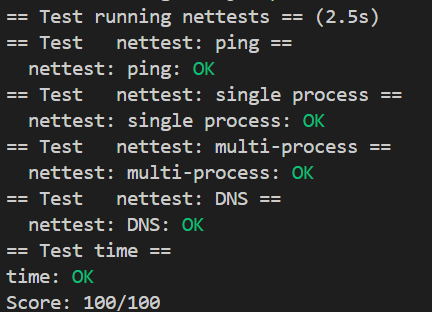
\includegraphics[width=\linewidth]{pics/net评测结果.png}
    \caption{评测结果}
    \label{fig:net}
\end{figure}

\subsection{实验小结}

通过本次实验,我成功实现了在xv6操作系统中对E1000网络设备的驱动程序编写。具体实现了数据包的发送(e1000\_transmit函数)和接收(e1000\_recv函数)功能。这一过程加深了我对设备驱动程序工作原理的理解,尤其是在网络通信中的应用。

整个实验过程中,我不仅掌握了如何编写和调试设备驱动程序,还通过实际操作理解了操作系统中网络通信的底层机制。这些经验和知识为我今后开发复杂的系统级软件奠定了坚实的基础。同时,通过评测脚本验证了我实现的正确性,确保了驱动程序的功能和性能达到了预期的目标。